% !TeX program = latexmk -lualatex
\documentclass[sigconf,nonacm,screen]{acmart}

\AtBeginDocument{%
  \providecommand\BibTeX{{%
    Bib\TeX}}}

\setcopyright{cc}
\setcctype{by-sa}
\copyrightyear{2024}

%----------------------------------------------------------------------------------------
%	Custom definitions and stuff
%----------------------------------------------------------------------------------------

\newcommand{\quotes}[1]{``#1''}
\newcommand{\squotes}[1]{`#1'}


\usepackage{tikz}
\usepackage{mathtools}
\usetikzlibrary{calc}
\usetikzlibrary{backgrounds}
\usepackage{multirow}

\usepackage{amsmath}
\usepackage{placeins} % for \FloatBarrier



% green version
\definecolor{color_circb_bg}{HTML}{053620}
\definecolor{color_circb_grid}{HTML}{2d7454}
\definecolor{color_circb_wire}{HTML}{88c441}
\definecolor{color_circb_wire_highlight}{HTML}{00cfff}
\definecolor{color_circb_metal}{HTML}{e2b677}
% \definecolor{color_circb_metal}{HTML}{000000}
\definecolor{color_marker_x}{HTML}{990099}
% \definecolor{color_marker_y}{HTML}{500050}
\colorlet{color_marker_y}{color_marker_x}
\definecolor{color_x_coords}{HTML}{aa0000}
\definecolor{color_y_coords}{HTML}{0000aa}
\definecolor{color_bounds}{HTML}{006437}
% \colorlet{color_bounds}{color_circb_bg}
\definecolor{color_contrast1}{HTML}{D00000}
\definecolor{color_contrast2}{HTML}{9d5aff}
\definecolor{color_contrast3}{HTML}{CCCCCC}
\definecolor{color_coordinate_labels}{HTML}{E0E0E0}
\definecolor{color_small_difference}{HTML}{A0A0A0}
% \definecolor{color_big_difference}{HTML}{000000}
\colorlet{color_big_difference}{color_marker_x}


\def\circbwirelinewidth{1mm}

\def\circbwire[#1](#2,#3,#4,#5){
    \draw[#1,line width=\circbwirelinewidth] (#2,#3) -- (#4,#5);
    \fill[#1] (#2,#3) circle (1.5mm);
    \fill[#1] (#4,#5) circle (1.5mm);
    \begin{pgfonlayer}{metallayer}
        \fill[color_circb_metal] (#2,#3) circle (1mm);
        \fill[color_circb_metal] (#4,#5) circle (1mm);
    \end{pgfonlayer}
}


\def\hdiffbracket[#1](#2,#3){
    \draw[#1,line width=0.25mm] (#2+0.04,11)--(#2+0.04,11.15)--(#2+#3-0.04,11.15)--(#2+#3-0.04,11);
    \node[#1] at (#2+#3/2,11.4) {$+#3$};
}
\def\vdiffbracket[#1](#2,#3){
    \draw[#1,line width=0.25mm] (11,#2+0.04)--(11.15,#2+0.04)--(11.15,#2+#3-0.04)--(11,#2+#3-0.04);
    \node[#1] at (11.48,#2+#3/2) {+#3};
}

\def\rowmarker(#1){
    \fill[color_marker_y] (-1.2, #1-0.25) -- (-0.8, #1) -- (-1.2, #1+0.25) -- (-1.125, #1);
}
\def\colmarker(#1){
    \fill[color_marker_y] (#1-0.25, -1.2) -- (#1, -0.8) -- (#1+0.25, -1.2) -- (#1, -1.125);
}

\def\circbmargin{.6}
\def\circbcornerradius{1mm}

\def\coordinatelabeloffset{-0.35}
\def\coordinatelabelsize{\tiny}

\newcommand{\todo}[1]{\textbf{\color{red}[TODO: #1]}}


% complexity
\newcommand{\bigO}{\mathcal{O}\hspace{-0.15em}}
\newcommand{\logs}{\log(s)}
\newcommand{\logw}{\log(w)}








\begin{document}

\title{Solving the ACM ICPC Problem \squotes{Wiring Assistant}}
\subtitle{% Scaling Down the Problem:
A Reduction Approach for Huge Grid Graphs}

\author{Samuel Füßinger}
\email{samuel.fuessinger@student.uni-tuebingen.de}
\affiliation{%
  \institution{Eberhard Karls Universität}
  \city{Tübingen}
  \state{Baden-Württemberg}
  \country{Germany}
  \postcode{72076}
}

\begin{abstract}
In this paper, we address the 2006 \emph{ACM International Collegiate Programming Contest} problem \squotes{Wiring Assistant}, which centers on finding the minimum path cost in potentially enormous grid graphs. We present an approach that can solve this problem efficiently by reducing the input grid graph through the removal of identical neighboring columns or rows, leading to a much more manageable size where pathfinding algorithms can be run in milliseconds. We prove that our reduction algorithm guarantees a worst-case grid size of $301\times303$. Additionally, we provide a detailed analysis of both the space and time complexity of our approach and examine its scalability limitations for the generalized problem without constraints on the maximum grid size and the number of wires.

Our full implementation is publicly available at \url{https://github.com/Samsu-F/Wiring_Assistant}.
\end{abstract}

\keywords{Pathfinding, Lattice path, A*-algorithm, Grid graph, ACM~ICPC, Wiring Assistant}

\maketitle

\section{Introduction}
\subsection{About ACM ICPC}
The \emph{ACM International Collegiate Programming Contest} (ICPC) is a global programming contest that challenges college students to efficiently solve algorithmically complex problems. Hosted annually by the \emph{Association for Computing Machinery} (ACM) since 1970, it aims to foster \quotes{collaboration, creativity, innovation, and the ability to perform under pressure} \cite{acm_icpc}.


\subsection{Problem}
In 2006, the ACM ICPC included a problem called \squotes{Wiring Assistant} \cite{wiring_assistant_problem}. In this problem, a circuit board composed of a grid of horizontal and vertical tracks is given, as well as a number of pre-existing wires running on these tracks. Additionally, two points that must be connected by a path on the grid are given (see Figure~\ref{fig:first_example} for an exemplary visualization).

Wires are strictly horizontal or vertical, running only on a single track. Horizontal and vertical wires may overlap in a single grid point. Two horizontal wires or two vertical wires may only overlap in their endpoints.

The tracks are numbered, starting from zero for the leftmost column and the bottom row. The wires are identified by the coordinates of their lower left endpoint followed by the upper right one. For example, Figure~\ref{fig:first_example} shows a possible scenario with the light green wires described by \texttt{~4~0~4~6 \ \ 0~5~6~5 \ \ 9~1~9~6 \ \ 7~4~7~7 \ \ 8~6~8~8 \ \ 4~6~6~6 \ \ 8~8~10~8}. The light blue points that need to be connected are described by the coordinates \texttt{7~8} and \texttt{6~1}.

% \verb|4 0 4 6  0 5 6 5  9 1 9 6  7 4 7 7  8 6 8 8  4 6 6 6  8 8 10 8|
\begin{figure}[h]
    \centering
    \begin{tikzpicture}[scale=0.6]
        % \fill[white, rounded corners=\circbcornerradius] (-0.5,-0.5) rectangle (10.5,10.5);
        % \pgfdeclarelayer{metallayer}
            \fill[color_circb_bg, rounded corners=\circbcornerradius] (-0\circbmargin,-0\circbmargin) rectangle (10\circbmargin,10\circbmargin);
            \draw[step=1.0,color_circb_grid,line width=0.1mm] (0,0) grid (10,10);
            \pgfdeclarelayer{metallayer}
            \pgfsetlayers{main,metallayer}
            \circbwire[color_circb_wire](4, 0, 4, 6)
            \circbwire[color_circb_wire](0, 5, 6, 5)
            \circbwire[color_circb_wire](9, 1, 9, 6)
            \circbwire[color_circb_wire](7, 4, 7, 7)
            \circbwire[color_circb_wire](8, 6, 8, 8)
            \circbwire[color_circb_wire](4, 6, 6, 6)
            \circbwire[color_circb_wire](8, 8, 10, 8)
            % the points to connect
            \fill[color_circb_wire_highlight] (7,8) circle (1.7mm);
            \fill[color_circb_wire_highlight] (6,1) circle (1.7mm);
            \begin{pgfonlayer}{metallayer}
                \fill[color_circb_metal] (7,8) circle (1mm);
                \fill[color_circb_metal] (6,1) circle (1mm);
            \end{pgfonlayer}
            % coordinate labels
            \foreach \x in {0,1,2,3,4,5,6,7,8,9,10}
                \node[color_coordinate_labels] at (\x, \coordinatelabeloffset) {\coordinatelabelsize $\x$};
            \foreach \y in {0,1,2,3,4,5,6,7,8,9,10}
                \node[color_coordinate_labels] at (\coordinatelabeloffset, \y) {\coordinatelabelsize $\y$};
    \end{tikzpicture}
    \caption{An example scenario with seven wires}
    \label{fig:first_example}
\end{figure}
\begin{figure}[h]
    \centering
    \begin{tikzpicture}[scale=0.6]
        % \fill[white, rounded corners=\circbcornerradius] (-0.5,-0.5) rectangle (10.5,10.5);
        % \pgfdeclarelayer{metallayer}
            \fill[color_circb_bg, rounded corners=\circbcornerradius] (-0\circbmargin,-0\circbmargin) rectangle (10\circbmargin,10\circbmargin);
            \draw[step=1.0,color_circb_grid,line width=0.1mm] (0,0) grid (10,10);
            \pgfdeclarelayer{metallayer}
            \pgfsetlayers{main,metallayer}
            \circbwire[color_circb_wire](4, 0, 4, 6)
            \circbwire[color_circb_wire](0, 5, 6, 5)
            \circbwire[color_circb_wire](9, 1, 9, 6)
            \circbwire[color_circb_wire](7, 4, 7, 7)
            \circbwire[color_circb_wire](8, 6, 8, 8)
            \circbwire[color_circb_wire](4, 6, 6, 6)
            \circbwire[color_circb_wire](8, 8, 10, 8)
            % the points to connect
            \draw[color_contrast1, line width=\circbwirelinewidth] (7,8) -- (7,1) -- (6,1);
            \draw[red, line width=0.5mm] (6.4,4.9) -- (7.6,6.1);
            \draw[red, line width=0.5mm] (6.4,6.1) -- (7.6,4.9);
            \draw[color_contrast2, line width=\circbwirelinewidth] (7,8) -- (5,8) -- (5,1) -- (6,1);
            % \draw[color_contrast2, line width=\circbwirelinewidth] (7,8) -- (6,8) -- (6,1);
            \draw[color_contrast3, line width=\circbwirelinewidth] (7,8) -- (7,9) -- (10,9) -- (10,0) -- (6,0) -- (6,1);
            \fill[color_circb_wire_highlight] (7,8) circle (1.7mm);
            \fill[color_circb_wire_highlight] (6,1) circle (1.7mm);
            \begin{pgfonlayer}{metallayer}
                \fill[color_circb_metal] (7,8) circle (1mm);
                \fill[color_circb_metal] (6,1) circle (1mm);
            \end{pgfonlayer}
            % coordinate labels
            \foreach \x in {0,1,2,3,4,5,6,7,8,9,10}
                \node[color_coordinate_labels] at (\x, \coordinatelabeloffset) {\coordinatelabelsize $\x$};
            \foreach \y in {0,1,2,3,4,5,6,7,8,9,10}
                \node[color_coordinate_labels] at (\coordinatelabeloffset, \y) {\coordinatelabelsize $\y$};
    \end{tikzpicture}
    \caption{Valid (light gray, purple) and invalid (red) paths for the scenario shown in Figure~\ref{fig:first_example}}
    \label{fig:example_valid_invalid_connections}
\end{figure}

For any given input, the objective is to calculate the minimum number of overlaps with existing wires for any path connecting the two given points. Overlaps with wire endpoints count as one overlap, just like overlaps with the middle of a wire. A path may not run on top of another wire but may overlap in single points.


For example, the purple path in Figure~\ref{fig:example_valid_invalid_connections} connects the points with two overlaps, while the light gray path connects them with only one overlap. There is no cheaper path connecting them with less than one overlap, making the integer \squotes{1} the correct solution for this scenario. Only the minimum number of overlaps needs to be found, it is not necessary to output the path.

The red path in Figure~\ref{fig:example_valid_invalid_connections} is invalid because it runs on top of the wire \texttt{~7~4~7~7}.

There are limits to the number of wires and the grid size.
The grid size, which is both the width and the height of the grid, of any given problem instance is a positive integer less than $10^{9}$. The number of wires is a positive integer less than $100$.

\subsection{Input Format}
The input is given in the form of three lines of plain text, containing decimal integers separated by spaces. The first line consists of the number of existing wires, and the size of the circuit board\footnote{i.e., the number of horizontal tracks, which is equal to the number of vertical tracks}. The second line contains --- in groups of four numbers per wire --- the coordinates of all wire endpoints. For each wire, the $x$- and $y$- coordinates of the lower left endpoint are given first, followed by the  $x$- and $y$- coordinates of the upper right endpoint. The third line contains the coordinates of the two points that need to be connected. To give an example, the problem instance shown in Figure~\ref{fig:first_example} could be described by the following input.
\begin{verbatim}
7 11
4 0 4 6 0 5 6 5 9 1 9 6 7 4 7 7 8 6 8 8 4 6 6 6 8 8 10 8
7 8 6 1
\end{verbatim}

% \FloatBarrier
\section{Outline of our Solution}
\subsection{Grid Graph Model} \label{subsection:grid_graph_model}
It is quite natural to think of this problem as a graph problem. Specifically, it can be interpreted as a problem on a square grid graph\footnote{A square grid graph is a lattice graph with square tiling. It does not imply that the graph itself is a square.}, where each point of the circuit board corresponds to a node of the graph. Each node has edges to its four immediate neighbors\footnote{i.e., $(x+1,y)$, $(x-1,y)$, $(x,y+1)$, and $(x,y-1)$}, except the nodes on the border and the corners, which have only three or two edges.
Each node is assigned a cost equal to the number of existing wires ending on or running through the corresponding point. For example, for the case shown in Figure~\ref{fig:first_example}, the node $(4,0)$ is assigned a cost of $1$, and $(4,5)$ has a cost of $2$.

We remove the edges of existing wires from the graph because an edge can be used for a new path if and only if there is no wire already present. 

Figure~\ref{fig:example_resulting_graph} illustrates this, showing the equivalent graph for the scenario depicted in Figure~\ref{fig:first_example}.

\begin{figure}[h]
    \centering
    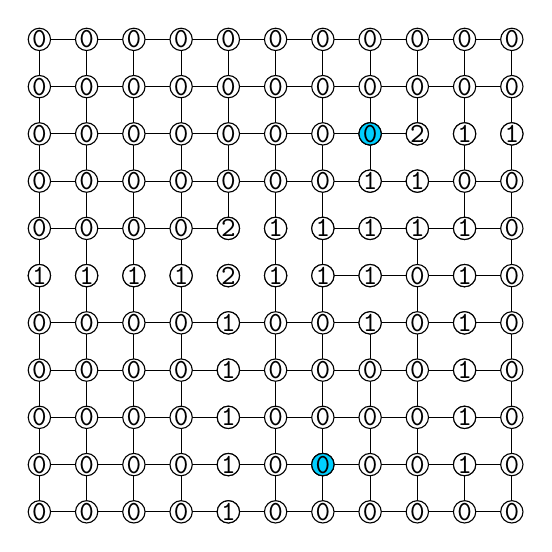
\begin{tikzpicture}[scale=0.6]
            % \fill[white, rounded corners=\circbcornerradius] (-0\circbmargin,-0\circbmargin) rectangle (10\circbmargin,10\circbmargin);
            % \pgfdeclarelayer{metallayer}
            \draw[step=1.0,black,line width=0.1mm] (0,0) grid (10,10);
            % eraser lines
            \draw[white, line width=1mm](4, 0) -- (4, 6);
            \draw[white, line width=1mm](0, 5) -- (6, 5);
            \draw[white, line width=1mm](9, 1) -- (9, 6);
            \draw[white, line width=1mm](7, 4) -- (7, 7);
            \draw[white, line width=1mm](8, 6) -- (8, 8);
            \draw[white, line width=1mm](4, 6) -- (6, 6);
            \draw[white, line width=1mm](8, 8) -- (10, 8);
            
            \foreach \x in {0,1,2,3,4,5,6,7,8,9,10}
                \foreach \y in {0,1,2,3,4,5,6,7,8,9,10}
                    \node[circle,draw, minimum size=2mm, inner sep=0pt, fill=white] at (\x,\y) {\texttt{0}};
            % nodes with a non-zero cost:
            \node[circle,draw, minimum size=2mm, inner sep=0pt, fill=white] at (4,0) {\texttt{1}};
            \node[circle,draw, minimum size=2mm, inner sep=0pt, fill=white] at (4,1) {\texttt{1}};
            \node[circle,draw, minimum size=2mm, inner sep=0pt, fill=white] at (4,2) {\texttt{1}};
            \node[circle,draw, minimum size=2mm, inner sep=0pt, fill=white] at (4,3) {\texttt{1}};
            \node[circle,draw, minimum size=2mm, inner sep=0pt, fill=white] at (4,4) {\texttt{1}};
            \node[circle,draw, minimum size=2mm, inner sep=0pt, fill=white] at (4,5) {\texttt{2}};
            \node[circle,draw, minimum size=2mm, inner sep=0pt, fill=white] at (4,6) {\texttt{2}};
            %
            \node[circle,draw, minimum size=2mm, inner sep=0pt, fill=white] at (0,5) {\texttt{1}};
            \node[circle,draw, minimum size=2mm, inner sep=0pt, fill=white] at (1,5) {\texttt{1}};
            \node[circle,draw, minimum size=2mm, inner sep=0pt, fill=white] at (2,5) {\texttt{1}};
            \node[circle,draw, minimum size=2mm, inner sep=0pt, fill=white] at (3,5) {\texttt{1}};
            % duplicate
            \node[circle,draw, minimum size=2mm, inner sep=0pt, fill=white] at (5,5) {\texttt{1}};
            \node[circle,draw, minimum size=2mm, inner sep=0pt, fill=white] at (6,5) {\texttt{1}};
            %
            \node[circle,draw, minimum size=2mm, inner sep=0pt, fill=white] at (9,1) {\texttt{1}};
            \node[circle,draw, minimum size=2mm, inner sep=0pt, fill=white] at (9,2) {\texttt{1}};
            \node[circle,draw, minimum size=2mm, inner sep=0pt, fill=white] at (9,3) {\texttt{1}};
            \node[circle,draw, minimum size=2mm, inner sep=0pt, fill=white] at (9,4) {\texttt{1}};
            \node[circle,draw, minimum size=2mm, inner sep=0pt, fill=white] at (9,5) {\texttt{1}};
            \node[circle,draw, minimum size=2mm, inner sep=0pt, fill=white] at (9,6) {\texttt{1}};
            %
            \node[circle,draw, minimum size=2mm, inner sep=0pt, fill=white] at (7,4) {\texttt{1}};
            \node[circle,draw, minimum size=2mm, inner sep=0pt, fill=white] at (7,5) {\texttt{1}};
            \node[circle,draw, minimum size=2mm, inner sep=0pt, fill=white] at (7,6) {\texttt{1}};
            \node[circle,draw, minimum size=2mm, inner sep=0pt, fill=white] at (7,7) {\texttt{1}};
            %
            \node[circle,draw, minimum size=2mm, inner sep=0pt, fill=white] at (8,6) {\texttt{1}};
            \node[circle,draw, minimum size=2mm, inner sep=0pt, fill=white] at (8,7) {\texttt{1}};
            \node[circle,draw, minimum size=2mm, inner sep=0pt, fill=white] at (8,8) {\texttt{2}};
            %
            % duplicate
            \node[circle,draw, minimum size=2mm, inner sep=0pt, fill=white] at (5,6) {\texttt{1}};
            \node[circle,draw, minimum size=2mm, inner sep=0pt, fill=white] at (6,6) {\texttt{1}};
            %
            % duplicate
            \node[circle,draw, minimum size=2mm, inner sep=0pt, fill=white] at (9,8) {\texttt{1}};
            \node[circle,draw, minimum size=2mm, inner sep=0pt, fill=white] at (10,8) {\texttt{1}};
            % points to connect
            \node[circle,draw, minimum size=2mm, inner sep=0pt, fill=color_circb_wire_highlight] at (7,8) {\phantom{\texttt{0}}};
            \node[circle,draw, minimum size=2mm, inner sep=0pt, fill=color_circb_wire_highlight] at (6,1) {\phantom{\texttt{0}}};
            \node[circle,draw, minimum size=2mm, inner sep=0pt, fill=color_circb_wire_highlight] at (7,8) {\texttt{0}};
            \node[circle,draw, minimum size=2mm, inner sep=0pt, fill=color_circb_wire_highlight] at (6,1) {\texttt{0}};
    \end{tikzpicture}
    \caption{The equivalent graph for the scenario shown in Figure~\ref{fig:first_example}}
    \label{fig:example_resulting_graph}
\end{figure}

We define the cost of a path as the sum of the node costs for all nodes on the path. Since the node cost is the number of intersecting wires for a node, it is easy to see that the cost of a path is equal to the number of overlaps with existing wires for the corresponding path on the circuit board. Consequently, the cost of the cheapest path between two given nodes is equal to the minimum number of overlaps for any connection of the given points on the printed circuit board, which is the number we want to calculate.

\subsection{Na\"ive Approach}
An intuitive subsequent approach would be to use a pathfinding algorithm like Dijkstra's algorithm or A* to calculate the cost of the cheapest path. However, the width and height of the input graph are only limited to be less than $10^9$, meaning the graph could have almost $10^{18}$ nodes. Figure~\ref{fig:naive_infeasible} shows an example where this would be a serious problem.
\begin{figure}[h]
    \centering
    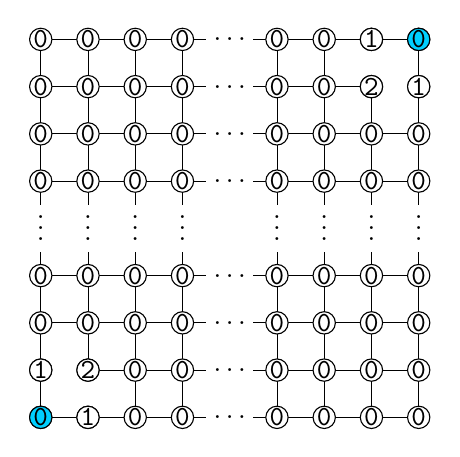
\begin{tikzpicture}[scale=0.6]
        % \fill[white, rounded corners=\circbcornerradius] (-0\circbmargin,-0\circbmargin) rectangle (10\circbmargin,10\circbmargin);
        % \pgfdeclarelayer{metallayer}
        \draw[step=1.0,black,line width=0.1mm] (0,0) grid (3.5,3.5);
        \draw[step=1.0,black,line width=0.1mm] (0,4.5) grid (3.5,8);
        \draw[step=1.0,black,line width=0.1mm] (4.5,0) grid (8,3.5);
        \draw[step=1.0,black,line width=0.1mm] (4.5, 4.5) grid (8,8);
        % eraser lines
        \draw[white, line width=1mm](0, 1) -- (1, 1);
        \draw[white, line width=1mm](1, 0) -- (1, 1);
        \draw[white, line width=1mm](8, 7) -- (7, 7);
        \draw[white, line width=1mm](7, 8) -- (7, 7);

        % all nodes
        \foreach \x in {0,1,2,3,5,6,7,8}
            \foreach \y in {0,1,2,3,5,6,7,8}
                \node[circle,draw, minimum size=2mm, inner sep=0pt, fill=white] at (\x,\y) {\texttt{0}};

        % dots
        \foreach \y in {0,1,2,3,5,6,7,8}
            \node at (4,\y) {$\ldots$};
        \foreach \x in {0,1,2,3,5,6,7,8}
            \node at (\x,4.18) {$\vdots$};
        
        % nodes with a non-zero cost:
        \node[circle,draw, minimum size=2mm, inner sep=0pt, fill=white] at (1,0) {\texttt{1}};
        \node[circle,draw, minimum size=2mm, inner sep=0pt, fill=white] at (0,1) {\texttt{1}};
        \node[circle,draw, minimum size=2mm, inner sep=0pt, fill=white] at (1,1) {\texttt{2}};
        \node[circle,draw, minimum size=2mm, inner sep=0pt, fill=white] at (7,8) {\texttt{1}};
        \node[circle,draw, minimum size=2mm, inner sep=0pt, fill=white] at (8,7) {\texttt{1}};
        \node[circle,draw, minimum size=2mm, inner sep=0pt, fill=white] at (7,7) {\texttt{2}};
        
        % points to connect
        \node[circle,draw, minimum size=2mm, inner sep=0pt, fill=color_circb_wire_highlight] at (0,0) {\texttt{0}};
        \node[circle,draw, minimum size=2mm, inner sep=0pt, fill=color_circb_wire_highlight] at (8,8) {\texttt{0}};
    \end{tikzpicture}
    \caption{A graph for which the na\"ive approach is infeasible}
    \label{fig:naive_infeasible}
\end{figure}
With a width and height of $999,999,999$ nodes and the wires
% $((0,1),(1,1)); (1,0),(1,1))$
\texttt{0~1~1~1} and \texttt{1~0~1~1},
as well as equivalent wires in the opposite corner, the \quotes{distance} --- i.e., the path cost --- from any of the nodes in the middle to a corner is strictly less than the minimum path cost for a connection of the corner nodes marked in blue. Therefore, if one were to calculate the cost of connecting the marked corners using Dijkstra's algorithm or A*, almost all of the nearly $10^{18}$ nodes would have to be visited. Even with the very optimistic estimation that visiting a node takes only a single CPU clock cycle, this would still result in a runtime of $7.9$~core years on a 4~GHz CPU!
So clearly, this na\"ive approach is not feasible.

\subsection{Our Reduction Approach}
Before any processing can be done, the input needs to be parsed. We parse line by line, number by number and store them into a simple struct with fields for the number of wires, the size, and the points to be connected; and an array field in which the coordinates of the wire endpoints are held. 

Unlike the na\"ive approach, our reduction approach then leverages the low number of wires to drastically decrease the problem size.

The number of wires is limited to a maximum of 99, so the vast majority of the circuit board tracks on large inputs are empty. This gives us an opportunity to greatly reduce the graph to a manageable size, without changing the minimum cost between nodes. The idea is relatively simple: identical neighboring columns or rows, that do not contain a wire endpoint, are redundant and can be combined into only one column or row. Figures~\ref{fig:redundant_tracks} and \ref{fig:combined_tracks} illustrate this; the minimum cost to connect any two points in Figure~\ref{fig:redundant_tracks} is the same as the one for the corresponding points in Figure~\ref{fig:combined_tracks}.
\begin{figure}[h]
    \centering
    \begin{tikzpicture}[scale=0.6]
        \fill[color_circb_bg, rounded corners=\circbcornerradius] (-0\circbmargin,-0\circbmargin) rectangle (10\circbmargin, 10\circbmargin);
        \draw[step=1.0,color_circb_grid,line width=0.1mm] (0,0) grid (10,10);
        \pgfdeclarelayer{metallayer}
        \pgfsetlayers{main,metallayer}
        \circbwire[color_circb_wire](4, 0, 4, 6)
        \circbwire[color_circb_wire](0, 5, 6, 5)
        \circbwire[color_circb_wire](9, 1, 9, 6)
        \circbwire[color_circb_wire](7, 4, 7, 7)
        \circbwire[color_circb_wire](8, 6, 8, 8)
        \circbwire[color_circb_wire](4, 6, 6, 6)
        \circbwire[color_circb_wire](8, 8, 10, 8)
        % % the points to connect
        % \fill[color_circb_wire_highlight] (7,8) circle (1.7mm);
        % \fill[color_circb_wire_highlight] (6,1) circle (1.7mm);
        % \begin{pgfonlayer}{metallayer}
        %     \fill[color_circb_metal] (7,8) circle (1mm);
        %     \fill[color_circb_metal] (6,1) circle (1mm);
        % \end{pgfonlayer}
        % % markers
        % \fill[color_marker_y] (-1.1, 1.8) -- (-0.8, 2) -- (-1.1, 2.2);
        \rowmarker(2)
        \rowmarker(3)
        \rowmarker(9)
        \rowmarker(10)
        \colmarker(1)
        \colmarker(2)
        \colmarker(3)
        
        % coordinate labels
        \foreach \x in {0,1,2,3,4,5,6,7,8,9,10}
            \node[color_coordinate_labels] at (\x, \coordinatelabeloffset) {\coordinatelabelsize $\x$};
        \foreach \y in {0,1,2,3,4,5,6,7,8,9,10}
            \node[color_coordinate_labels] at (\coordinatelabeloffset, \y) {\coordinatelabelsize $\y$};
        % diff markers
        \hdiffbracket[color_big_difference](0,4)
        \vdiffbracket[color_big_difference](1,3)
        \vdiffbracket[color_big_difference](8,3)
        
        \vdiffbracket[color_small_difference](-1,1)
        \vdiffbracket[color_small_difference](0,1)
        \vdiffbracket[color_small_difference](4,1)
        \vdiffbracket[color_small_difference](5,1)
        \vdiffbracket[color_small_difference](6,1)
        \vdiffbracket[color_small_difference](7,1)
        
        \hdiffbracket[color_small_difference](-1,1)
        \hdiffbracket[color_small_difference](4,2)
        \hdiffbracket[color_small_difference](6,1)
        \hdiffbracket[color_small_difference](7,1)
        \hdiffbracket[color_small_difference](8,1)
        \hdiffbracket[color_small_difference](9,1)
        \hdiffbracket[color_small_difference](10,1)
    \end{tikzpicture}
    \caption{A problem instance with redundant rows and columns (indicated by the purple pointers)}
    \label{fig:redundant_tracks}
\end{figure}
\begin{figure}[h]
    \centering
    % \begin{tikzpicture}[scale=0.6]
    %     \fill[color_circb_bg, rounded corners=\circbcornerradius] (-0.5,-0.5) rectangle (10.5,10.5);
    %     % \draw[step=1.0,color_circb_grid,line width=0.1mm] (0,0) grid (10,10);
    %     \foreach \x in {0,2,4,5,6,7,8,9,10}
    %         \draw[color_circb_grid,line width=0.1mm] (\x,0) grid (\x,10);
    %     \foreach \y in {0,1,2,4,5,6,7,8,10}
    %         \draw[color_circb_grid,line width=0.1mm] (0,\y) grid (10,\y);
    %     \pgfdeclarelayer{metallayer}
    %     \pgfsetlayers{main,metallayer}
    %     \circbwire[color_circb_wire](4, 0, 4, 6)
    %     \circbwire[color_circb_wire](0, 5, 6, 5)
    %     \circbwire[color_circb_wire](9, 1, 9, 6)
    %     \circbwire[color_circb_wire](7, 4, 7, 7)
    %     \circbwire[color_circb_wire](8, 6, 8, 8)
    %     \circbwire[color_circb_wire](4, 6, 6, 6)
    %     \circbwire[color_circb_wire](8, 8, 10, 8)
    %     % the points to connect
    %     \fill[color_circb_wire_highlight] (7,8) circle (1.7mm);
    %     \fill[color_circb_wire_highlight] (6,1) circle (1.7mm);
    %     \begin{pgfonlayer}{metallayer}
    %         \fill[color_circb_metal] (7,8) circle (1mm);
    %         \fill[color_circb_metal] (6,1) circle (1mm);
    %     \end{pgfonlayer}
    %     % % markers
    %     % \fill[color_marker_y] (-1, 1.8) -- (-0.7, 2) -- (-1, 2.2);
    %     % \fill[color_marker_y] (-1, 2.8) -- (-0.7, 3) -- (-1, 3.2);
        
    %     % \fill[color_marker_y] (-1, 9.8) -- (-0.7, 10) -- (-1, 10.2);
    %     % \fill[color_marker_y] (-1, 8.8) -- (-0.7, 9) -- (-1, 9.2);
        
    %     % \fill[color_marker_x] (0.8, 11) -- (1, 10.7) -- (1.2, 11);
    %     % \fill[color_marker_x] (1.8, 11) -- (2, 10.7) -- (2.2, 11);
    %     % \fill[color_marker_x] (2.8, 11) -- (3, 10.7) -- (3.2, 11);
    % \end{tikzpicture}
    \begin{tikzpicture}[scale=0.6]
        \fill[color_circb_bg, rounded corners=\circbcornerradius] (-0\circbmargin,-0\circbmargin) rectangle (8\circbmargin,8\circbmargin);
        \draw[step=1.0,color_circb_grid,line width=0.1mm] (0,0) grid (8,8);
        \pgfdeclarelayer{metallayer}
        \pgfsetlayers{main,metallayer}
        \circbwire[color_circb_wire](2, 0, 2, 5)
        \circbwire[color_circb_wire](0, 4, 4, 4)
        \circbwire[color_circb_wire](7, 1, 7, 5)
        \circbwire[color_circb_wire](5, 3, 5, 6)
        \circbwire[color_circb_wire](6, 5, 6, 7)
        \circbwire[color_circb_wire](2, 5, 4, 5)
        \circbwire[color_circb_wire](6, 7, 8, 7)
        % the points to connect
        % \fill[color_circb_wire_highlight] (7,8) circle (1.7mm);
        % \fill[color_circb_wire_highlight] (6,2) circle (1.7mm);
        % \begin{pgfonlayer}{metallayer}
        %     \fill[color_circb_metal] (7,8) circle (1mm);
        %     \fill[color_circb_metal] (6,2) circle (1mm);
        % \end{pgfonlayer}
        % coordinate labels
        \foreach \x in {0,1,2,3,4,5,6,7,8}
            \node[color_coordinate_labels] at (\x, \coordinatelabeloffset) {\coordinatelabelsize $\x$};
        \foreach \y in {0,1,2,3,4,5,6,7,8}
            \node[color_coordinate_labels] at (\coordinatelabeloffset, \y) {\coordinatelabelsize $\y$};
    \end{tikzpicture}
    \caption{The same problem instance as in Figure~\ref{fig:redundant_tracks}, with the redundant tracks merged.}
    \label{fig:combined_tracks}
\end{figure}

The implementation of this idea is straightforward and should be run before transforming the input into a graph representation as outlined in Section~\ref{subsection:grid_graph_model}.
It can be accomplished with the help of two arrays, one containing the $x$-coordinates and the other one containing the $y$-coordinates of all wire endpoints. The arrays are sorted and subsequently iterated over, identifying differences~$d$ between consecutive values equal to or greater than three. As illustrated in Figure~\ref{fig:redundant_tracks}, such a difference of $d\geq3$ is found if and only if there are two or more consecutive columns or rows between these coordinates that do not contain any wire endpoints. By subtracting $d-2$ from all of the remaining coordinates after the gap, the redundant columns or rows are effectively removed (cf. Figure~\ref{fig:combined_tracks}). Attention should be paid to ensure that potential redundancies at the edges of the circuit board are also removed and that the given points to connect are placed back on the correct coordinates. Our implementation ensures both of these points rather trivially by including the width and height of the circuit board, as well as the coordinates of the points to connect, in the respective array. \label{subsection:incl_points_to_connect_in_arrays} This simple and computationally cheap solution does, however, come at the cost of a slightly larger worst-case size of the reduced circuit board (see Section~\ref{subsection:effectiveness_reduction} for details).

After reducing the input problem instance as described, it is transformed into a graph representation (as explained in Section~\ref{subsection:grid_graph_model}) that allows for the efficient execution of the pathfinding algorithm. We chose to represent the graph with two matrices: one saving the cost for each node, while the other contains four-bit bit-vectors that indicate whether there is an edge in the positive and negative $x$- and $y$-directions for each node. For example, the least significant bit represents the edge in the positive $x$-direction, so \verb|neighbors[x][y]| has this bit set if and only if there is an edge connecting the node at $(x,y)$ to the node at $(x+1,y)$.

As the pathfinding algorithm, we opted for the A*-algorithm, since knowing the coordinates of both the start and end node allows us to gauge in which direction the path search appears most promising. As the metric of an arbitrary node to the start node, we use a tuple $(cost, distance)$, where the cost is the sum of all node costs traversed on the path as defined previously. The distance is simply the number of edges on the path. Metrics are compared lexicographically, i.e., $(c_1,d_1) < (c_2,d_2)$ if and only if $c_1 < c_2$ or $c_1 = c_2 \wedge d_1 < d_2$\footnote{This comparison can be efficiently implemented by interpreting the tuple as an unsigned integer, wherein the cost occupies the most significant bits and the distance occupies the least significant bits.}.

For the heuristic function that estimates the metric for a node~$n$ to the goal~$g$, we use $h(n) = (0, d(n,g))$, where $d(n,g)$ is the Manhattan distance from $n$ to the goal node. This means we estimate that reaching the goal is possible without crossing any more wires and in the shortest distance possible. Clearly, this heuristic is admissible, i.e., it cannot overestimate the actual metric to reach the goal. It is also consistent, meaning that traveling one node further can never decrease the heuristic by more than the metric increase that resulted from the step just taken.

A notable alteration from the conventional A*-algorithm is that we do not record the predecessor nodes, since we are not interested in reconstructing the shortest path, but only in its cost\footnote{Our implementation offers an optional \texttt{-p} flag, with which the predecessor nodes are tracked and the path is reconstructed and displayed. However, this is only for demonstration and not necessary for the ACM ICPC problem.}.

\subsection{Effectiveness of the Reduction} \label{subsection:effectiveness_reduction}
Note: The calculations in this section are based on the simple solution (as described in Section~\ref{subsection:incl_points_to_connect_in_arrays}) that includes the width and height of the circuit board, as well as the coordinates of the points to connect, in the arrays used to identify redundant tracks. This is also the version implemented in the code belonging to this paper. A marginal improvement of the worst-case size is possible with a more sophisticated algorithm, but we chose to stick with this simpler, albeit slightly worse, version for ease of understanding and consistency of paper and implementation.

Since the previously described reduction algorithm removes redundant tracks, i.e., neighboring columns or rows that both do not contain any given points\footnote{By \emph{given points}, we mean the wire endpoints, the start, and the goal.}, there cannot be two neighboring rows or columns that both do not contain any given points after running the reduction. Therefore, the worst-case size of the circuit board after the reduction is a width of double the number of unique $x$-coordinates plus one, and analogously for the height with the number of unique $y$-coordinates. For example, in Figure~\ref{fig:worst_case_two_wires}, there are five unique $x$-coordinates and five unique $y$-coordinates, each of them having had one or more empty rows and columns to all sides before the reduction.
This results in a width and height of $2 \cdot 5 + 1 = 11$, and thus $11^2=121$ nodes, which is the worst-case size for the case of two wires.

\begin{figure}[h]
    \centering
    \begin{tikzpicture}[scale=0.6]
        \fill[color_circb_bg, rounded corners=\circbcornerradius] (-0\circbmargin,-0\circbmargin) rectangle (10\circbmargin,10\circbmargin);
        \draw[step=1.0,color_circb_grid,line width=0.1mm] (0,0) grid (10,10);
        \pgfdeclarelayer{metallayer}
        \pgfsetlayers{main,metallayer}
        \circbwire[color_circb_wire](1,1,1,3)
        \circbwire[color_circb_wire](5,7,7,7)
        % the points to connect
        \fill[color_circb_wire_highlight] (3,5) circle (1.7mm);
        \fill[color_circb_wire_highlight] (9,9) circle (1.7mm);
        \begin{pgfonlayer}{metallayer}
            \fill[color_circb_metal] (3,5) circle (1mm);
            \fill[color_circb_metal] (9,9) circle (1mm);
        \end{pgfonlayer}
        % coordinate labels
        \foreach \x in {0,1,2,3,4,5,6,7,8,9,10}
            \node[color_coordinate_labels] at (\x, \coordinatelabeloffset) {\coordinatelabelsize $\x$};
        \foreach \y in {0,1,2,3,4,5,6,7,8,9,10}
            \node[color_coordinate_labels] at (\coordinatelabeloffset, \y) {\coordinatelabelsize $\y$};
    \end{tikzpicture}
    \caption{The worst case size after the reduction for the case of two wires.}
    \label{fig:worst_case_two_wires}
\end{figure}

With this knowledge of the worst-case width and height, we can infer that the worst-case number of nodes is $width \cdot height = (2\cdot |\textit{unique x-coordinates}|+1) \cdot (2\cdot|\textit{unique y-coordinates}|+1)$.

Since each wire is either horizontal or vertical (and not diagonal), either its $x$-coordinates or its $y$-coordinates are identical, meaning each wire can have up to three unique coordinate components. The start and end point can also contribute up to two unique coordinate components each%\footnote{With a more sophisticated algorithm it would be possible to ignore these four coordinate components (also see Section~\ref{subsection:incl_points_to_connect_in_arrays}).}
.
We know that there are no more than $99$ wires, therefore, we have at most $3 \cdot 99 + 2 \cdot 2 = 301$ unique components.

We can find an upper limit for the product $width \cdot height$ by looking at the sum $width + height$ first:
\begin{align*}
    &\phantom{=~} width + height\\
    &=(2\cdot|\textit{unique x-coordinates}|+1)+(2\cdot|\textit{unique y-coordinates}|+1)\\
    &= 2\cdot(|\textit{unique x-coordinates}|+|\textit{unique y-coordinates}|)+2\\
    &= 2\cdot(|\textit{unique components}|)+2\\
    &\leq 2\cdot301+2\\
    &= 604
\end{align*}
Since the product of any two natural numbers is less than or equal to the square of their arithmetic mean\footnote{a direct consequence of the AM--GM inequality}, it follows logically that $width \cdot height \leq {\left(\frac{width + height}{2}\right)}^2 = {\left(\frac{604}{2}\right)}^2 = 302^2 = 91204$. As in the worst-case both $width$ and $height$ are odd numbers, the true upper bound on the number of nodes is actually $301 \cdot 303 = 91203$ nodes, which is many orders of magnitude smaller than the possibly close to $10^{18}$ nodes we had before the reduction.

More generally speaking, a problem instance with $w$~wires has at most $3\cdot w + 4$ unique coordinate components, so after the reduction, both the width and the height are in $\bigO\left(w\right)$ and the resulting graph will not have more than ${\left(\frac{2\cdot(3\cdot w+4)+2}{2}\right)}^2 = (3w+5)^2$ nodes.

\section{Performance Analysis} \label{section:performance_analysis}
Given that the original problem as set in the competition has upper limits on both the number of wires and the size of the circuit board, the number of unique problem instances is finite.
Consequently, the complexity (both in space and time) of any algorithm solving it is in $\mathcal{O}(1)$
as there is a constant time in which any of the finite number of possible inputs can be solved.

Because this does not provide meaningful insights, in this section, we analyze the complexity of a generalized version of the problem without limits on the size of the circuit board and the number of wires. From now on, unless marked otherwise, the discussed complexities are worst-case complexities in big O notation dependent on the grid size~$s$ and the number of wires~$w$.

As the grid size~$s$ grows arbitrarily large, so does the number of digits of $s$, albeit only logarithmically. To store $s$, you need at least $\log_2(s+1)$~bits of memory, which affects the space and time required if $s$ grows arbitrarily large. Since the maximum value for coordinates is obviously limited by the grid size, their number of bits is already accounted for in $\logs$.
% we do not need to consider their number of digits separately but can treat them the same as $s$.
As shown in Section~\ref{subsection:effectiveness_reduction}, the size after the reduction step is in $\bigO\left(w\right)$, meaning its number of bits needed to store the size is in $\bigO\left(\logw\right)$.
Note that $\bigO\left(\logw\right) \subset \bigO\left(\logs\right)$, since $w<2s^2$ (as there cannot be more wires than edges).
This automatically introduces a factor of $\logs$ for any piece of code that processes coordinates or the grid size before or during the reduction step, and a factor of $\logw$ for any code handling coordinates or the size after the reduction.

\subsection{Complexity Step by Step}
Both the time and space complexity of parsing the input are proportional to the number of wires~$w$ multiplied with the aforementioned $\log(s)$ factor for the coordinates' growing number of digits. Therefore, they are in $\bigO\left(w\cdot\logs\right)$, which is another way of saying they are linearly bounded by the number of characters in the input string.

The reduction step requires sorting the wire endpoint coordinates, which can be achieved in $\bigO\left(w\cdot\log(w)\right)$ time with linear space complexity\footnote{for example with heapsort or mergesort}. All other subtasks of the reduction step --- which are splitting the coordinates into the two arrays and later iterating over the sorted arrays to identify gaps --- can be accomplished in linear space and time\footnote{for an arbitrary but fixed $s$, otherwise there is the additional $\logs$ factor}. This leaves us with a time complexity of $\bigO\left(w\cdot\log(w)\cdot\logs\right)$ and a space complexity of $\bigO\left(w\cdot\logs\right)$ for the reduction step\footnote{In our implementation, we use the C standard library function \emph{qsort}, which --- despite its name --- has no complexity guarantees. The actual space and time complexities are implementation specific~\cite{cppreference_qsort}. The latest GNU C Library version at the time of writing uses mergesort with heapsort as a fallback \cite{glibc}.}.

% Building the graph requires setting up a matrix storing whether there is an edge for each node adjacent in the grid. As there are at most four adjacent nodes for every node in the grid, both the time and space complexity of this task are in $\bigO\left(|V|)$\footnote{ignoring the $\log$-factor for the growing number of digits needed to identify the nodes}, where $V$ is the set of all nodes. In Section~\ref{subsection:effectiveness_reduction} we saw that the number of nodes after the reduction is quadratically bounded by $w$ and it is obviously not greater than the original number of nodes\footnote{Note that for large values of $w$, $\bigO\left(s^2)$ is a tighter constraint than $\bigO\left(w^2)$, since $w$ itself is in $\bigO\left(s^2)$.}, giving us a space and time complexity of $\bigO\left(\min(w^2,s^2)\cdot\logw)$ for constructing this matrix.

% The other matrix storing the cost of each node can be set up by filling it with zeros first, then iterating over all wires, for each wire iterating over all nodes it passes through and incrementing the cost for each node. Since the length of each wire is obviously limited by the width or height respectively, which are themselves linearly bounded by the number of wires (see Section~\ref{subsection:effectiveness_reduction}), the resulting space and time complexities for constructing this cost matrix are also $\bigO\left(w^2\cdot\logs)$, making them the total complexities for building the graph.

Building the graph requires setting up two matrices, one storing the cost of each node and the other one storing whether there is an edge for each node adjacent in the grid. This can be achieved by iterating over all wires, for each wire iterating over all nodes it passes through, while incrementing the cost for each node and deleting each edge it passes through. As wires cannot be stacked, we can visit each node at most four times and each edge at most once.  Therefore, both the time and space complexity of this step are in $\bigO\left(|E|\right)=\bigO\left(|V|\right)$\footnote{ignoring the $\log$-factor for the growing number of digits needed to identify the nodes}, where $V$ is the set of all nodes and $E$ is the set of all edges. In Section~\ref{subsection:effectiveness_reduction}, we saw that the number of nodes after the reduction is quadratically bounded by $w$ and it is obviously not greater than the original number of nodes\footnote{Note that for large values of $w$, $\bigO\left(s^2\right)$ is a tighter constraint than $\bigO\left(w^2\right)$ since $w$ itself is in $\bigO\left(s^2\right)$.}, giving us a space and time complexity of $\bigO\left(\min(w^2,s^2)\cdot\logw\right)$ for constructing these matrices.

The A*-algorithm performs a loop iteration for each metric--node pair queued. Per loop iteration one pair has to be dequeued and up to three neighbors get enqueued into the priority queue, taking $\bigO\left(\log(n)\cdot\logw\right)$ time\footnote{The $\logw$-factor is once again there because of the growing number of digits.}, where $n$ is the number of elements in the queue. Each node cannot possibly get enqueued more times than the number of edges it has, %\todo: Beleg einfügen
i.e., not more than four times. This means there are $\bigO\left(|V|\right)$ many loop iterations, each taking a time of $\bigO\left(\log(|V|)\cdot\logw\right)$. Just like in the previous step, we can substitute $|V|$ with $\min(w^2,s^2)$, resulting in a time of \\$\bigO\left(\min(w^2,s^2)\cdot\log(w^2)\cdot\logw\right)$
% = \bigO\left(\min(w^2,s^2)\cdot2\log(w)\cdot\logw\right)
$= \bigO\left(\min(w^2,s^2)\cdot\log^2(w)\right)$ for A*.

A*'s space is in $\bigO\left(|V|\cdot\logw\right) = \bigO\left(\min(w^2,s^2)\cdot\logw\right)$, because both the priority queue and the matrix that is used to save the metrics need to save a constant number of metrics (each of size $\logw$) per node.


% \begin{table}[h]
%     \centering
%     \begin{tabular}{|l|c|c|}
%         \cline{2-3}
%         \multicolumn{1}{c|}{}       & \textbf{Time}                                        & \textbf{Space}                    \\ \hline
%         \textbf{Parsing}            & $\bigO\left(w\cdot\logs\right)$                      & $\bigO\left(w\cdot\logs\right)$ \\ \hline
%         \textbf{Reduction}          & $\bigO\left(w\cdot\log(w)\cdot\logs\right)$          & $\bigO\left(w\cdot\logs\right)$ \\ \hline
%         \textbf{Building the Graph} & $\bigO\left(\min(w^2,s^2)\cdot\logw\right)$          & $\bigO\left(\min(w^2,s^2)\cdot\logw\right)$ \\ \hline
%         \textbf{A$\mathbf{^*}$}     & $\bigO\left(\min(w^2,s^2)\cdot\log^2(w)\right)$      & $\bigO\left(\min(w^2,s^2)\cdot\logw\right)$ \\ \hline
%         \hline
%         %                           & $\bigO(\max($                                        & $\bigO(\max($ \\
%         % \textbf{Total}            & $\phantom{\bigO(\max(}w\cdot\log(w)\cdot\logs,$      & $\phantom{\bigO(\max(}w\cdot\logs$ \\
%         %                           & $\phantom{\bigO(\max(}\min(w^2,s^2)\cdot\log^2(w)$   & $\phantom{\bigO(\max(}\min(w^2,s^2)\cdot\logw$ \\
%         %                           & $)$                                                  & $)$ \\
%         \textbf{Total}
%             &   \multicolumn{1}{|c|}{
%                     \begin{minipage}{0cm}
%                         \setlength{\jot}{0pt} % Adjust spacing between lines of align
%                         \begin{align*}
%                                 \bigO\left(\max\left(\right.\right.~ & \\
%                                                                      & w\cdot\log(w)\cdot\logs, \\
%                                                                      & \min(w^2,s^2)\cdot\log^2(w) \\
%                                 ))\phantom{\bigO\max~}               &
%                         \end{align*}
%                     \end{minipage}
%                 }
%             &   \multicolumn{1}{|c|}{
%                     \begin{minipage}{0cm}
%                         \setlength{\jot}{0pt} % Adjust spacing between lines of align
%                         \begin{align*}
%                                 \bigO\left(\max\left(\right.\right.~ & \\
%                                                                      & w\cdot\logs, \\
%                                                                      & \min(w^2,s^2)\cdot\logw \\
%                                 ))\phantom{\bigO\max~}               &
%                         \end{align*}
%                     \end{minipage}
%                 }
%             \\
%         \hline
%     \end{tabular}
%     \caption{Space and time complexity}
%     \label{table:complexity_overview}
% \end{table}
\begin{table}[h]
    \centering
    \begin{tabular}{lc}
        % \multicolumn{1}{c|}{}       & \textbf{Time}                                      \\
        \toprule
        Parsing            & $\bigO\left(w\cdot\logs\right)$                    \vphantom{${X^X_X}^X_X$}\vspace{1mm} \\
        Reduction          & $\bigO\left(w\cdot\log(w)\cdot\logs\right)$        \vphantom{${X^X_X}^X_X$}\vspace{1mm} \\
        Building the Graph & $\bigO\left(\min(w^2,s^2)\cdot\logw\right)$        \vphantom{${X^X_X}^X_X$}\vspace{1mm} \\
        A$\mathbf{^*}$     & $\bigO\left(\min(w^2,s^2)\cdot{\log}^2(w)\right)$  \vphantom{${X^X_X}^X_X$}\vspace{1mm} \\
        % \hline
        \midrule
        \vspace{-5mm}\\
        Total
            &   \multicolumn{1}{c}{
                    \begin{minipage}{4cm}
                        \setlength{\jot}{0pt} % Adjust spacing between lines of align
                        \begin{align*}
                                \bigO\left((\right. &\hspace{-0.5mm} w\cdot\log(w)\cdot\logs ~+  \\
                                                    &\hspace{-0.5mm} \min(w^2,s^2)\cdot\log^2(w)) \vphantom{\underset{X}{X}}
                                % ))\phantom{\bigO\max~}               &
                        \end{align*}
                    \end{minipage}
                }
            \\
        \bottomrule
    \end{tabular}
    \caption{Time complexity}
    \label{table:time_complexity}
    \vspace{-5mm}
\end{table}
\begin{table}[h]
    \centering
    \begin{tabular}{lc}
        % \multicolumn{1}{c|}{}       & \textbf{Space}                              \\
        \toprule
        Parsing            & $\bigO\left(w\cdot\logs\right)$             \vphantom{${X^X_X}^X_X$}\vspace{1mm} \\
        Reduction          & $\bigO\left(w\cdot\logs\right)$             \vphantom{${X^X_X}^X_X$}\vspace{1mm} \\
        Building the Graph & $\bigO\left(\min(w^2,s^2)\cdot\logw\right)$ \vphantom{${X^X_X}^X_X$}\vspace{1mm} \\
        A*                 & $\bigO\left(\min(w^2,s^2)\cdot\logw\right)$ \vphantom{${X^X_X}^X_X$}\vspace{1mm} \\
        % \hline \hline
        % \setlength{\arrayrulewidth}{1mm} \hline
        \midrule
        \vspace{-5mm}\\
        Total
            &   \multicolumn{1}{c}{
                    \begin{minipage}{4cm}
                        \setlength{\jot}{0pt} % Adjust spacing between lines of align
                        \begin{align*}
                                \bigO\left(\right. &\hspace{-0.5mm} w\cdot\logs ~+           \\
                                                   &\hspace{-0.5mm} \min(w^2,s^2)\cdot\logw) \vphantom{\underset{X}{X}}
                                % )\phantom{\bigO~}  &
                        \end{align*}
                    \end{minipage}
                }
            \\
        \bottomrule
    \end{tabular}
    \caption{Space complexity}
    \label{table:space_complexity}
    \vspace{-5mm}
\end{table}

Table~\ref{table:time_complexity} and Table~\ref{table:space_complexity} give an overview of the complexities discussed. Of course, the total complexity of our solution is the sum of all the steps. It is particularly noteworthy that a huge grid size~$s$ has very little effect on the required space and time, affecting only the parsing and reduction steps negligibly. 




\section{Discussion of our Implementation}

\subsection{Programming Language}
We chose to implement our solution in the C programming language. Mainly, because C is one of the fastest, if not \emph{the} fastest widely used general-purpose language today \cite{10.1145/3125374.3125382}\cite{Fourment2008}\cite{PEREIRA2021102609}\footnote{This decision was also influenced by our personal preference and familiarity with C.}.

C's language design, most notably pointers, enabled some elegant solutions. For example, in C it is possible to iterate over an array of pointers, reading and changing the values at the locations pointed to. This is helpful if the values to be read or changed are different fields of different kinds of structs because it would not be possible to fill an array with different data types. To give an example, the \texttt{reduce} function in our implementation makes use of this possibility.

However, C also has some drawbacks. The lack of built-in high-level data structures, such as the priority queue needed for the A* algorithm, made implementing our solution much more time-consuming than we suspect it would have been in other languages.

In hindsight, while C was an appropriate choice, the extremely low execution times achieved were not really necessary for the purpose of demonstrating our algorithm. Thus, using a higher-level programming language with greater ease of use would also have been an appropriate option, despite the performance drawbacks.

\subsection{Scalability and its Limits}
For all problem instances of the original problem (i.e., grid size $s<10^{9}$ and number of wires $w\leq99$), our implementation solves each problem in at most a few milliseconds. However, when considering the generalized problem without these constraints, we run into the limits of data types and available time and memory. 

From the moment of parsing, through the reduction until the problem instance is transformed into the graph representation, the width and height of the grid, as well as all the coordinates, are stored in the \texttt{int\_fast32\_t} data type, defined in the C standard library \emph{stdint}. Their exact size is architecture- and compiler-dependent, but they are guaranteed to have at least 32 bits \cite{isoiec_C99}. Therefore, their maximum value could be as low as $2^{31}-1=2,147,483,647$, making this the maximum input grid size our implementation is guaranteed to work on.

The number of wires is stored as an \texttt{int}, making $2^{15}-1=32,767$ the maximum number of wires for which the behavior of our program is defined \cite{isoiec_C99}. However, in order to fit into an \texttt{uint16\_t}, the size after the reduction has to be smaller than $2^{16}$, which depends on the placement of the wires. For an arbitrary wire placement, this is only guaranteed to be the case for at most $2^{14}-2$~wires\footnote{because the width and height after the reduction can be up to $4\cdot w + 5$ (cf. Section~\ref{subsection:effectiveness_reduction})}. Note that while such a case can be solved by our implementation, the quadratic complexity (cf. Section~\ref{section:performance_analysis}) might make this infeasible, depending on the wire placement and how hard it is to find the cheapest path.

Another limit to consider is memory space. While running the A*-algorithm, up to twelve bytes\footnote{Note that we assume a byte to be eight bits for the following explanation.} of memory might be needed per node for the worst case\footnote{Two bytes per node for the graph representation, six bytes for the key--value pair in the priority queue, and four bytes in the \texttt{g\_scores} table.}. With $2^{14}-2$ wires, this could translate to up to $27.0$~GiB\footnote{$(3\cdot(2^{14}-2)+5)^2\cdot12 \mathrm{~bytes} = 28,989,849,612 \mathrm{~bytes}$} of memory. However, with dense wire placement and an easy-to-find path, a case with $2^{14}-2$~wires could require as little as approximately 48.5~KiB\footnote{with $76\times109$ nodes: $76\cdot109\cdot(2~\mathrm{bytes}+4~\mathrm{bytes})= 49704~\mathrm{bytes}$} to solve.

Stack space is not a concern for our implementation, as our sole recursive function\footnote{\texttt{\_pq\_heapify\_node}, used for the priority queue} is tail recursive and exhibits only a logarithmic recursion depth.



\section{Conclusion}
In this paper, we tackled the challenge of a potentially enormous input grid graph, developing a technique to reduce the graph through the removal of identical neighboring columns or rows, since they do not change the cost of the cheapest path. For the original ICPC problem, we found that our reduction technique guarantees a graph size of at most $301\times303$. For the generalized version of the problem, our analysis revealed that the space and time complexity of our approach is quasi-quadratic in the number of wires~$w$, while the input grid size~$s$ contributes only a logarithmic factor, extending the realm of what is feasible far beyond what is imaginable with a na\"ive approach.

Future research could explore finding more techniques to reduce the grid even further, as well as adapting pathfinding algorithms specialized for grid graphs, such as jump point search, to the specific characteristics of this problem.


\bibliographystyle{ACM-Reference-Format}
\bibliography{references}

\end{document}
\endinput
